% !TeX encoding = UTF-8
% !TeX spellcheck = en_US
\documentclass[a4paper,12pt]{article}
\usepackage[utf8]{inputenc}
\usepackage[english]{babel}
\usepackage{url}
\usepackage[colorlinks]{hyperref}
\usepackage{array}
\usepackage{arydshln}
%\usepackage{amsmath}
%\usepackage{array}
%\usepackage{arydshln}
\usepackage{multirow}
\usepackage{amsmath}
\usepackage{amsfonts}
\usepackage{amssymb}
\usepackage{graphicx}
\usepackage{subcaption}
\usepackage{amsthm}
\usepackage[scaled]{helvet}
\usepackage{algorithm}
\usepackage{algorithmicx}
\usepackage{algpseudocode}

\renewcommand\familydefault{\sfdefault} 
\usepackage[T1]{fontenc}

% \renewcommand{\baselinestretch}{1.5} 

\makeatletter
\newcommand\footnoteref[1]{\protected@xdef\@thefnmark{\ref{#1}}\@footnotemark}
\makeatother

\numberwithin{equation}{section}
\renewcommand{\thefootnote}{\fnsymbol{footnote}}

\theoremstyle{remark}
\newtheorem*{important}{Important}
\newtheorem*{recap}{Recap}

% macros
\newcommand{\eg}{e.g.,}
\newcommand{\ie}{i.e.,}
\newcommand{\FoR}{F.o.R.}
\newcommand{\SLAM}{SLAM}
\newcommand{\Slam}{Simultaneous Localization And Mapping}
\newcommand{\EKF}{EKF}
\newcommand{\Ekf}{Extended Kalman Filter}

\newcommand{\vect}[1]{\boldsymbol{\mathrm{{#1}}}}
\newcommand{\bvect}[1]{\bar{\vect{#1}}}

\newcommand{\notationAlert}{Here we write $\alpha \leftarrow f(\alpha)$ as a simplified notation for $\alpha_t = f(\alpha_{t-1})$, where $\alpha$ is any variable to be updated according to the value it had during the previous computational step and $t$ ranges over computational steps.}

%opening
\title{
	\textbf{
		\Slam{} via \Ekf{}
	} \\
	{\normalsize\textit{
		An informal tutorial for the \emph{Intelligent Robotic Systems} course
	}}
}
\author{
	Giovanni \textsc{Ciatto} \\ \texttt{giovanni.ciatto@studio.unibo.it} \\
}
\date{A.Y. 2015/2016}

\begin{document}
	
	\maketitle
	
	\section{Introduction}
		In the context of robotics, \Slam{} (\SLAM) is the problem of a robot dynamically constructing a map of an unknown environment and concurrently localizing itself within it, while exploring such environment. 
It may seem a chicken-or-egg problem, since a map is needed for localization and a frame of reference is needed for building a map, but the problem has been studied and solved both from a theoretical (probabilistic) and practical point of view in \cite{thrun2005}.

\SLAM{} involves a robotic agent being at least able to move within, and gather information about, the environment. Wheels and laser scanners are common choices to satisfy such requirements. 
Generally speaking, we will refer to them as \emph{actuators} and \emph{exteroceptive sensors}, respectively. 
Optionally, the robot may be equipped with one or more \emph{odometric} sensors allowing it to actually measure its own movement, which should otherwise be inferred, \eg{} by the speed imposed to the wheels. 
Generally speaking we call them \emph{proprioceptive sensors}. 

It is well understood in robotics that sensory data and inferred movement information are inherently noisy. 
From a probabilistic point of view this means that, if the robot is keeping track of its own position, the \emph{uncertainty} of about such position increases as the robot moves. 
Conversely, supposing the robot is able to detect some objects (\emph{landmarks}, in jargon) within its surroundings, recognize them for a number of observations, and estimate the relative position between itself and each landmark, then it can use such information to reduce the uncertainty about its own position.
Such a correlation between position estimation and landmark measurement is clearly explained in \cite[Unit C]{brenner204}.

The generic approach to \SLAM{} requires the following models to be properly defined: 
\begin{description}
	\item[Motion model:] describes how the robot updates the estimation of its own position and orientation according to the proprioceptive sensor data. 
	It depends on the degrees of freedom of the robot and the nature of the available data. 
	For instance, in this report, we consider the case of a differential robot constrained to move on a plane. 
	So the robot pose variables are $x$, $y$ and $\theta$ (the \emph{bearing}, in jargon) and the proprioceptive data consist of the last velocity values $v_l$ and $v_r$ imposed to the wheels motors.

	\item[Inverse Observation model:] describes how exteroceptive sensor data is used to deduce the landmarks positions, taking into account the current estimation of the robot position and orientation too.
	It depends on the nature of the data and the number of dimensions required to localize a landmark on the map.
	For example, in this report, we consider the case of a laser sensor providing, for each landmark, both its distance and angle w.r.t. the laser sensor.
	So the exteroceptive data consist of $(\rho,\, \alpha)$ pairs, which are used to deduce the landmark position $(x_m,\, y_m)$ on the map.
	
	\item[Direct Observation model:] describes how to predict the expected exteroceptive sensor data for a known landmark.
	From a conceptual point of view, it's the inverse function of the Inverse Observation model. 
	E.g., for our concerns, the Direct Observation Model takes into account the current estimation of the robot position and orientation $(x,\, y,\, \theta)$ and some known landmark position $(x_m,\, y_m)$ and computes the expected sensor data $(\rho,\, \alpha)$.
\end{description}
		
	\section{Models and Reference Frames}
		\begin{figure}
	\centering
	\begin{subfigure}[b]{.58\textwidth}
		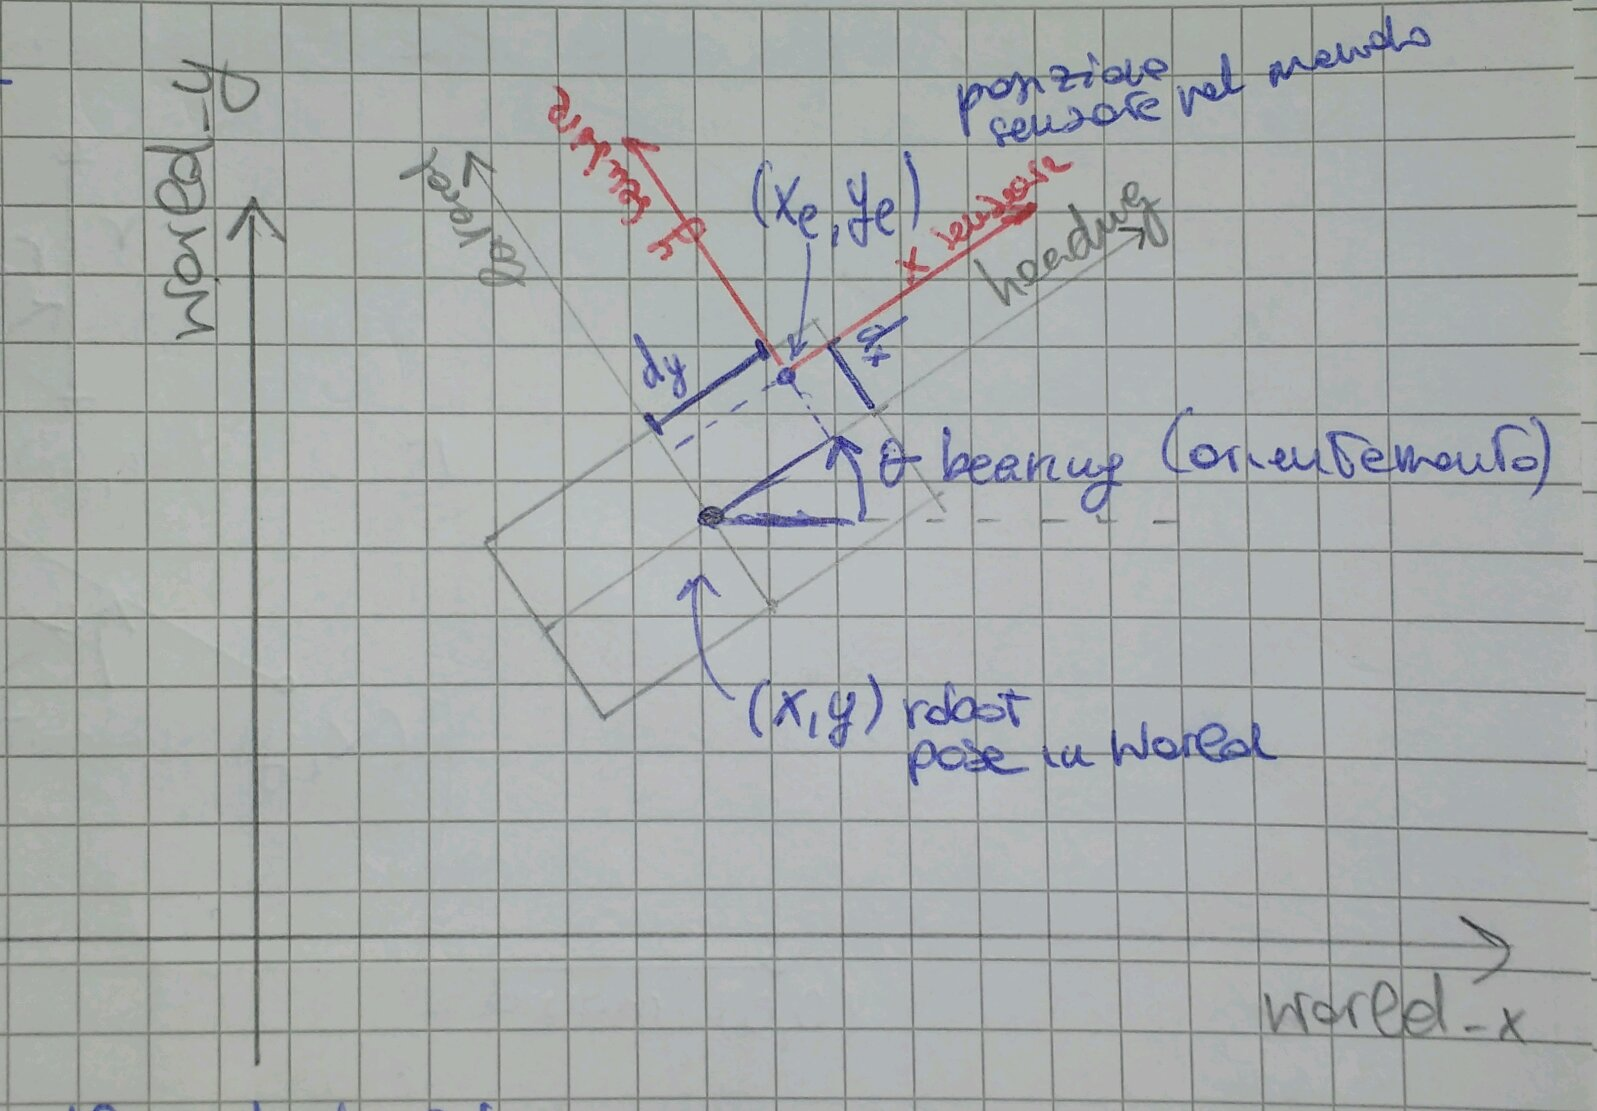
\includegraphics[width=\linewidth]{./img/frames_of_reference.png}
		\caption{The \emph{sensor} \FoR{}, inside the \emph{robot} \FoR{}, inside the \emph{map} \FoR{}.}
		\label{fig.fors.nested}
	\end{subfigure}
	\hfill
	\begin{subfigure}[b]{.38\textwidth}
		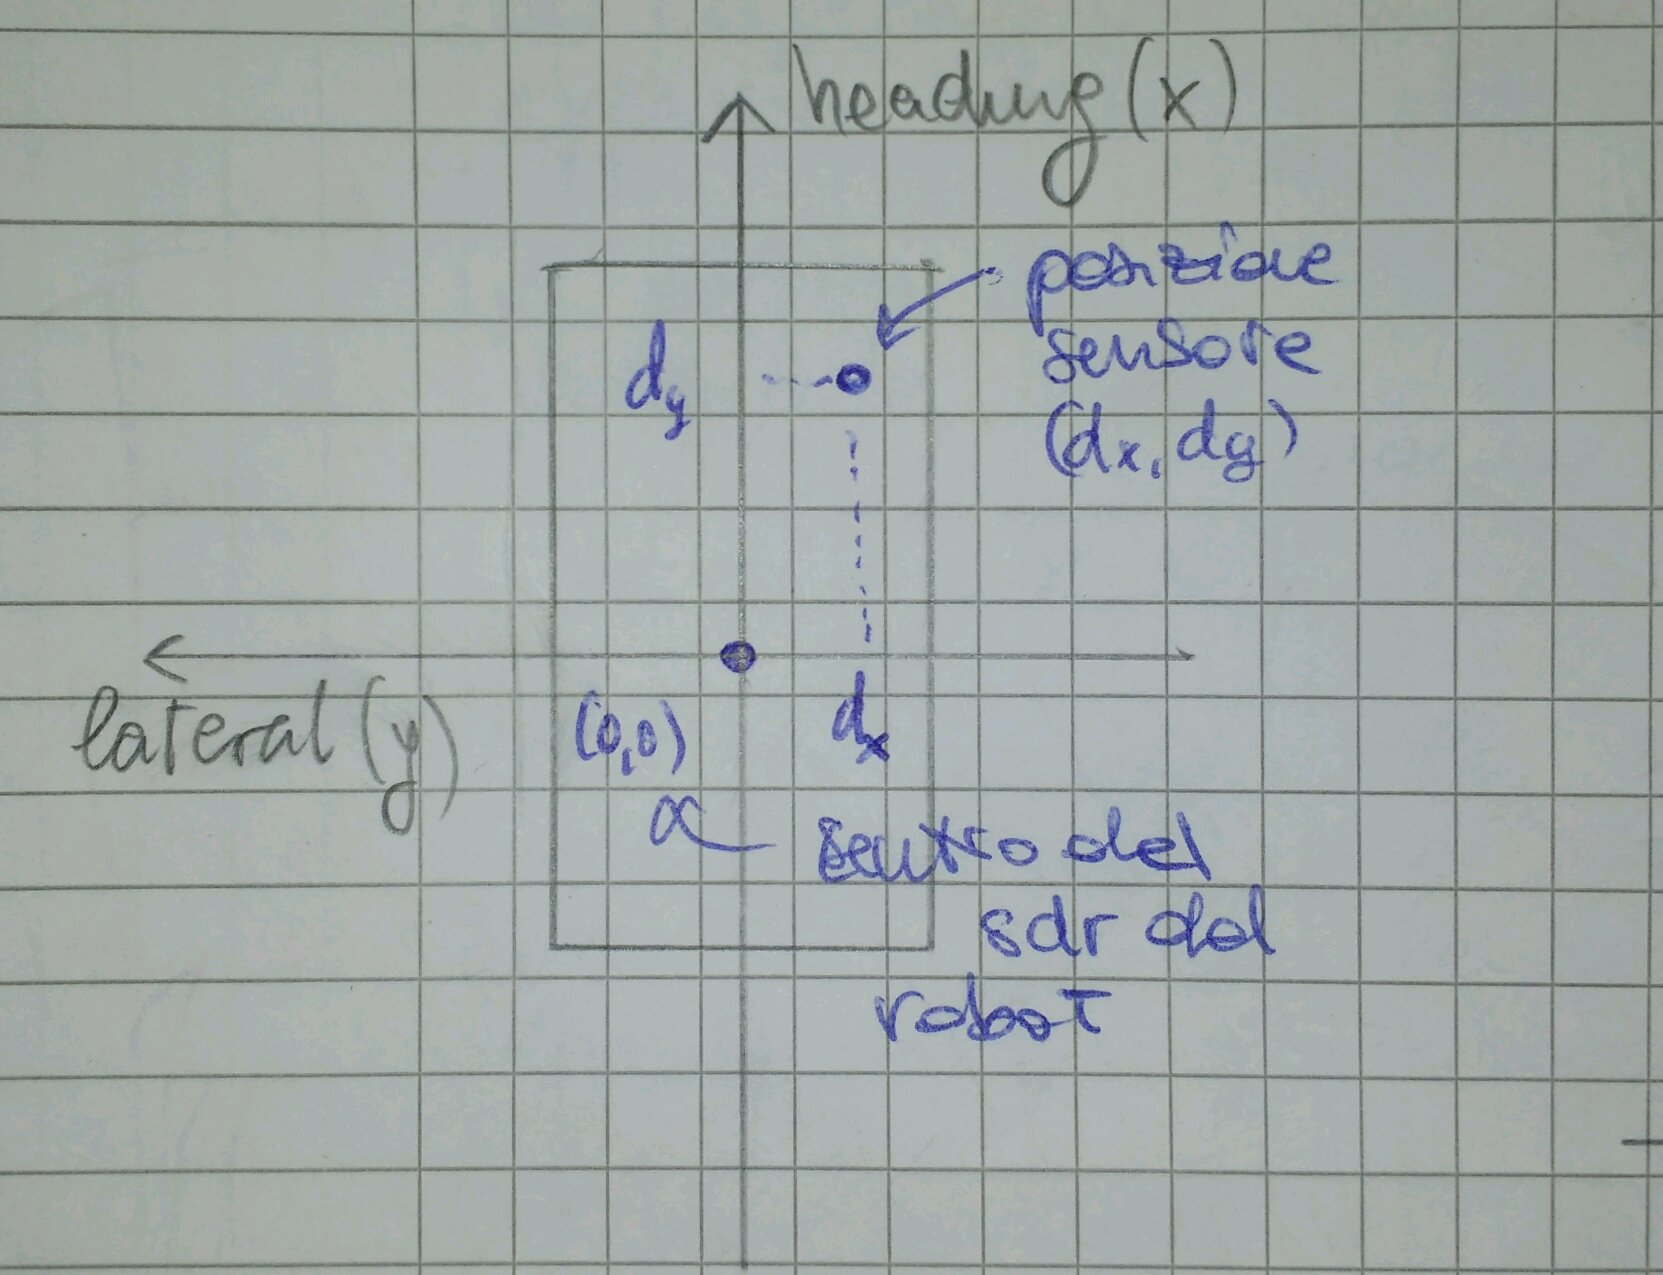
\includegraphics[width=\linewidth]{./img/robot_for.png}
		\caption{The \emph{robot} \FoR{} and the sensor position within it.}
		\label{fig.fors.robot}
	\end{subfigure}
	\caption{Frames of references (\FoR) considered the SLAM problem.}
	\label{fig.fors}
\end{figure}

It is important to understand that several Frames of Reference (\FoR{}) are involved in \SLAM{} (as shown in Figure \ref{fig.fors}):
\begin{itemize}
	\item The \emph{map} (or \emph{global}) \FoR{}, \ie{} the one used for representing the map and the current robot orientation and position. 
	It is arbitrary.
	
	\item The \emph{robot} (or \emph{local}) \FoR{}, \ie{} the one defined according to the reference center of the robot. 
	For what concerns this report, we consider a frame having its origin into the robot geometry center, the abscissas axis always coinciding with the heading direction, and the ordinate axis coinciding with the lateral direction (increasing on the left, as shown in Figure \ref{fig.fors.robot}).
	
	\item The \emph{sensor} (or \emph{measurement}) \FoR{}, which depends on the exteroceptive sensor position within the robot frame, and is in general different from the robot frame. 
	E.g., the sensor may be in position $(d_x,\, d_y)^\top$ w.r.t. the robot frame, as shown in Figure \ref{fig.fors.robot}, and this translation should be taken into account when handling sensor data in order to understand obstacles position on the map.
	In this tutorial we consider, for simplicity, the sensor frame to be coincident with the robot frame \ie{} $d_x = d_y = 0$.
	
\end{itemize}

Please note that, since part of the SLAM process is to build a map of the environment under the hypothesis that the robot has no prior knowledge about it, there is no constraint on how the robot should choose the initial global frame.
In what follows, we (and the robot) assume that the global frame coincides with the initial robot frame, \ie{} the map frame is defined by the initial pose of the robot into the environment: the origin is its \emph{very first} position, the abscissas axis is its \emph{initial} heading direction and, consequently, the ordinate axis is its \emph{initial} lateral direction.

\subsection{The motion model}
	The motion model is a function $g : \mathbb{R}^n \times \mathbb{R}^m \rightarrow \mathbb{R}^n$ mapping the previous robot pose vector, $\vect{r}_{t-1} \in \mathbb{R}^n$, \ie{} the vector containing the robot position and orientation (which are relative to the \emph{map} frame), into the current one, $\vect{r}_t \in \mathbb{R}^n$, by taking into account the last \emph{control} vector $\vect{u}_t \in \mathbb{R}^m$, \ie{} the vector containing proprioceptive data (which is relative to the \emph{robot} frame). More formally:
	\[
		\vect{r}_t = g(\vect{r}_{t-1},\, \vect{u}_t)
	\]
	
	\paragraph{Example: Differential robot on the plane.}
		Suppose we only own a two-wheeled, differential robot having no odometric sensor, which is often the case in experimental setups.
		The distance between the wheels is $2L$.
		Suppose we want to experiment the SLAM problem on planar arena containing some obstacles.
		Finally, suppose that each step of the robot controller is executed after ${\Delta T}_t$ seconds since the end of the previous step and that the duration of each step is negligible.
		Under such assumptions, movements relative to the $z$-axis are not so relevant: we are only interested in the robot to solve the SLAM problem on the 2D plane.
		In this setting we can assume the robot pose vector to be the triplet $\vect{r}_t = (x_t,\, y_t,\, \theta_t)^\top$, \ie{} the position and bearing of the robot w.r.t. the global frame, and the control vector to be the triplet $\vect{u}_t = (v_{l,t},\, v_{r,t},\, {\Delta T}_t)^\top$, \ie{} the velocities imposed to the wheels actuators at the end of the previous control step and the time elapsed since that moment.
		Notice that, if we assume ${\Delta T}_t$ to be constant, the control vector is the pair $\vect{u}_t = (v_{l,t},\, v_{r,t})^\top$.
		Under such hypotheses, the motion model could be defined as follows\footnote{\label{sec.models.alert}\notationAlert}:
		\begin{equation}
			\label{eq.motion.differential}
			\left(\begin{array}{c}
				x \\ y \\ \theta
			\end{array}\right)
			\leftarrow
			\left(\begin{array}{ccc}
				\cos{\theta} & -\sin{\theta} & 0 \\
				\sin{\theta} & \cos{\theta} & 0 \\
				0 & 0 & 1
			\end{array}\right)
			\cdot {\Delta T} \cdot I \cdot
			\left(\begin{array}{c}
				\frac{v_l + v_r}{2} \\ 
				0 \\
				\frac{v_r - v_l}{2L}
			\end{array}\right)
			+
			\left(\begin{array}{c}
				x \\ y \\ \theta
			\end{array}\right)
		\end{equation}
		where ${\Delta T} \cdot I$ is a diagonal $3 \times 3$ matrix having each element on the diagonal equal to ${\Delta T}$.
		Equation \ref{eq.motion.differential} computes the translation and rotation the robot performed within its reference frame during the last control step as a function of the velocity imposed to the wheels. 
		Such values are converted into the map frame and added to the previous position and orientation in order to achieve the new ones. 
		
		Please consider reading Appendix \ref{app.affine2d} and \ref{app.differential_drive} in order to recall conversions between reference frames and differential drive.
		
	\paragraph{Example: The odometric sensor.}
		Suppose our robot is embodied with an odometric sensor, which periodically provides a triplet $(dh,\, dl, d\theta)^\top$, \ie{} the variations in the heading and lateral directions and the angular variation since the last update. 
		Such variations are of course relative to the robot frame.
		We assume such a sensor frequency to be high.
		In this case the motion model could be simply defined as follows\footnoteref{sec.models.alert}:
		\begin{equation}
			\label{eq.motion.odometrix}
			\left(\begin{array}{c}
				x \\ y \\ \theta
			\end{array}\right)
			\leftarrow
			\left(\begin{array}{ccc}
				\cos{\theta} & -\sin{\theta} & 0 \\
				\sin{\theta} & \cos{\theta} & 0 \\
				0 & 0 & 1
			\end{array}\right)
			\cdot
			\left(\begin{array}{c}
				dh \\
				dl \\
				d\theta
			\end{array}\right)
			+
			\left(\begin{array}{c}
				x \\ y \\ \theta
			\end{array}\right)
		\end{equation}
		This means the variations relative to the robot frame are simply converted into the map frame.
		
	\section{\Ekf{} Phases}
		\label{sec.ekf_phases}
		In this section we describe and motivate the \EKF{} algorithm allowing us to face the \SLAM{} problem.

\subsection{The system state}
	Here we define the concept of (system) \emph{state}, which will be pervasively used in the following.
	
	The system state $\vect{x}_t$ consist of the robot pose vector $\vect{r}_t$ and the position vector $\vect{m}_{1},\, \vect{m}_{2},\, \ldots,\, \vect{m}_{M}$ of each known landmark. It is indeed defined as the concatenation of such vectors:
	\[
		\vect{x}_t \stackrel{def}{=}
		\left(\begin{array}{c}
			\vect{r}_t \\ \vect{m}_{1} \\ \vect{m}_{2} \\ \vdots \\ \vect{m}_{M}
		\end{array}\right)
		=
		\left(\begin{array}{c}
			\vect{r}_t \\ \vect{m}
		\end{array}\right)
		\in \mathbb{R}^{n + M \cdot q}
	\]
	where $\vect{m} \in \mathbb{R}^{M \cdot q}$ is a compact way to express the concatenation of all the known landmarks position vectors.
	
	The purpose of the \EKF-\SLAM{} algorithm is to produce and update an estimation of the state vector exploiting the exteroceptive and proprioceptive data. 
	It is important to understand that the robot \emph{cannot} know its exact state because of the noise afflicting sensors and actuators.
	Hence, we assume the state to be a multi-normal random vector (please refer to Appendix \ref{app.multinormal} for details) for which we assume to know the initial mean $\bvect{x}_0$ and covariances matrix $\Sigma_0$.
	The \EKF-\SLAM{} algorithm allows to compute the mean $\bvect{x}_t$ and covariances matrix $\Sigma_t$ of the current state as a function of the mean $\bvect{x}_{t - 1}$ and covariances matrix $\Sigma_{t - 1}$ of the previous state.
	The mean $\bvect{x}_t$ represents the most recent estimation of the robot pose and landmarks positions, while the covariances matrix $\Sigma_t$ stores the uncertainty of such estimation.
	
	Generally speaking, the mean and covariances are in the following form:
	\[
		\bvect{x}_t =
		\left(\begin{array}{c}
			\bvect{r}_t \\ \bvect{m}_{1,t} \\ \bvect{m}_{2,t} \\ \vdots \\ \bvect{m}_{M,t}
		\end{array}\right)
		=
		\left(\begin{array}{c}
			\bvect{r}_t \\ \bvect{m}_t
		\end{array}\right)
		\in \mathbb{R}^{n + M \cdot q}
	\]
	(notice that the expected position $\bvect{m}_{i,t}$ of any landmark may vary --- \ie{} be corrected --- as time progresses, while the actual position $\vect{m}_{i}$ is supposed not to change)
	\[
		\Sigma_t =
		\left(\begin{array}{cc}
			\sigma_{\vect{r},\vect{r}, t} & \sigma_{\vect{r},\vect{m}, t} \\
			\sigma_{\vect{m},\vect{r}, t} & \sigma_{\vect{m},\vect{m}, t}
		\end{array}\right)
		\in \mathcal{M}_{(n + M \cdot q) \times (n + M \cdot q)}(\mathbb{R})
	\]
	where $\sigma_{\vect{r},\vect{r}, t} \in \mathcal{M}_{n \times n}(\mathbb{R})$ is the sub-matrix containing the covariances of the pose, $\sigma_{\vect{r},\vect{m}, t} \in \mathcal{M}_{n \times M \cdot q}(\mathbb{R})$ is the sub-matrix containing the covariances of the pose w.r.t. the landmark positions,  $\sigma_{\vect{m},\vect{r}, t} = \sigma^\top_{\vect{r},\vect{m}, t}$, since $\Sigma_t$ must be symmetric, and $\sigma_{\vect{m},\vect{m}, t} \in \mathcal{M}_{M \cdot q \times M \cdot q}(\mathbb{R})$ is the sub-matrix containing the covariances of the landmark positions.
	
	Please notice that $M$, \ie{} the number of currently known and mapped landmarks, may actually vary as the robot moves, since more landmarks may be discovered.
	
	\subsubsection{The initial state}
	
		As stated before, we (and the robot) assume that the global frame coincides with the robot frame at the very first step of the \SLAM{} algorithm. We also assume that the robot has no prior knowledge about the landmarks positions, \ie{} $M_0 = 0$.
		This implies that:
		\[
			\bvect{x}_0 = \bvect{r}_0 = \vect{0}
			\hspace{2cm}
			\Sigma_0 = \vect{0}
		\]
		meaning that the robot is supposed to have \emph{null uncertainty} about its initial position to be the origin of the global frame.
		
		In what follows we will explain:
		\begin{itemize}
			\item How $\bvect{x}_t$ and $\Sigma_t$ can be extended when a measurement vector $\vect{s}$ detects an unknown landmark
			\item How $\bvect{x}_t$ and $\Sigma_t$ can be computed as functions of $\bvect{x}_{t-1}$ and $\Sigma_{t-1}$, taking into account the last control vector $\vect{u}_t$ and some measurement vector $\vect{s}$ relative to some known landmark
		\end{itemize}
		
\subsection{The system and observation errors}
	TODO write this
		
\subsection{The prediction phase}
	In the prediction phase the motion model $g(\cdot)$ is exploited to produce an estimation of the current robot state $\bvect{x}_t$ taking into account the previous robot state $\bvect{x}_{t-1}$ and the last control vector $\bvect{u}_t$.
	The uncertainty about the system state $\Sigma_t$ is computed accordingly.
	
	Conceptually, this step is simple: the robot just needs to compute\footnote{\label{sec.ekf.alert}\notationAlert}
	\[
		\vect{x} \leftarrow f(\vect{x},\, \vect{u})
	\]
	where $f$ is the function applying the motion model to the first $n$ components of $\vect{x}$ and leaving the others unchanged\footnoteref{sec.ekf.alert}:
	\[
		\vect{x} = 
		\left(\begin{array}{c}
			\vect{r} \\ \vect{m}
		\end{array}\right)
		\leftarrow
		\left(\begin{array}{c}
			g(\vect{r},\, \vect{u}) \\ \vect{m}
		\end{array}\right) 
		= f(\vect{x},\, \vect{u})
	\]
	Sadly, the robot never knows the \emph{real} system state or control vector or landmark positions, but it only knows their means and covariances as multi-normal variables.
	Mathematically, this step is complicated by $g(\cdot)$ being, in general, non-linear.
	So, while applying a linear transformation to some multi-normal variables moments, as explained in Appendix \ref{app.multinormal}, surely produces two multi-normal variable moments; applying a non-linear transformation does not guarantee so.
	This limitation is overcome by linearizing the $f$ function into the point $(\bvect{x}_{t-1},\, \bvect{u}_{t})^\top$ as explained in Appendix \ref{app.jacobian}.
	
	Hence, the predicted robot state mean $\bvect{x}_t$ is computed as follows\footnoteref{sec.ekf.alert}:
	\begin{equation}
		\label{eq.prediction.mean.update}
		\bvect{x} = 
		\left(\begin{array}{c}
			\bvect{r} \\ \bvect{m}
		\end{array}\right)
		\leftarrow
		\left(\begin{array}{c}
			g(\bvect{r},\, \bvect{u}) \\ \bvect{m}
		\end{array}\right)
		= f(\bvect{x},\, \bvect{u})
	\end{equation}
	assuming that the robot motion do not affect the landmark positions.
	
	Linearizing $f$ allows us to compute the predicted robot state covariances matrix $\Sigma_t$.
	Such step is usually presented as follows\footnoteref{sec.ekf.alert}:
	\begin{equation}
		\label{eq.prediction.sigma.jacobians}
		\Sigma_t = F_{\vect{x}} \cdot \Sigma_{t-1} \cdot F^\top_{\vect{x}} \ + \ F_{\vect{u}} \cdot E \cdot F^\top_{\vect{u}}
	\end{equation}
	where $F_{\vect{x}} = \partial f(\bvect{x}_{t-1},\, \bvect{u}_{t}) / \partial \vect{x}$ and $F_{\vect{u}} = \partial f(\bvect{x}_{t-1},\, \bvect{u}_{t}) / \partial \vect{u}$ are the Jacobians of the $f$ function into the point $(\bvect{x}_{t-1},\, \bvect{u}_{t})^\top$ w.r.t. the system state and the control, respectively. 
	
	Since we assumed the $f$ function not affecting the landmarks positions, Equation \ref{eq.prediction.sigma.jacobians} reduces to the following update rules\footnoteref{sec.ekf.alert}:
	\begin{equation}
		\label{eq.prediction.covs.update.rr}
		\sigma_{\vect{r},\vect{r}} \leftarrow G_{\vect{r}} \cdot \sigma_{\vect{r},\vect{r}} \cdot G^\top_{\vect{r}} \ + \ G_{\vect{u}} \cdot E \cdot G^\top_{\vect{u}}
	\end{equation}
	\begin{equation}
		\label{eq.prediction.covs.update.rm}
		\sigma_{\vect{r},\vect{m}} \leftarrow G_{\vect{r}} \cdot \sigma_{\vect{r},\vect{m}}
	\end{equation}
	\begin{equation}
		\label{eq.prediction.covs.update.mr}
		\sigma_{\vect{m},\vect{r}} \leftarrow \sigma^\top_{\vect{r},\vect{m}}
	\end{equation}
	\begin{equation}
		\label{eq.prediction.covs.update.mm}
		\sigma_{\vect{m},\vect{m}} \leftarrow \sigma_{\vect{m},\vect{m}}
	\end{equation}
	
		
	\section{Algorithm for \Slam{}}
		In this section we unify the phases described in Section \ref{sec.ekf_phases} into a single algorithm which can be employed as a starting point for solving the \SLAM{} problem.

Algorithm \ref{alg.ekf.step} shows the pseudocode of the $t$-th step of the \Ekf{}.
Each phase from Section \ref{sec.ekf_phases} is encapsulated within a function call.
Here we consider the general (and usual) case where a set of measurements $S$ relative to the $t$-th step is available.
Measurement vectors in $S$ contribute to the correction phase one after another.

Only one algorithmic step per control vector should be executed, \ie{} the \textsc{Ekf\_Step} should be called as soon as a new control vector is available: calling it more frequently would be a waste of computational resources.
Moreover, if the control vector source is an odometric sensor, it is important to keep the execution time of the $t$-th step lower than the time between two consecutive sensor data, otherwise the robot estimated state will become inconsistent.
This may be critical since the robot will supposedly keep discovering new landmarks, increasing both the space and time required to execute one step of the algorithm.

\begin{algorithm}
	\caption{\Ekf{} $t$-th step}
	\label{alg.ekf.step}
	\begin{algorithmic}[1]
		
		\Function{Ekf\_Step}{$\bvect{x}$, $\Sigma$, $M$, $\bvect{u}$, $S$}
%			\Statex
			\State $\bvect{x}$, $\Sigma$ $\gets$ \Call{Prediction}{$\bvect{x}$, $\Sigma$, $\bvect{u}$}
%			\Statex
			\ForAll{$\bvect{s} \in S$}
%				\Statex
				% \State $\bvect{m}$ $\gets$ \Call{Inverse\_Observation}{$\bvect{x}$, $\bvect{s}$}
				\State $i$, $\bvect{m}$ $\gets$ \Call{Recognition}{$\bvect{x}$, $\Sigma$, $\bvect{s}$}
%				\Statex
				\If {$i = M + 1$}
					\State $\bvect{x}$, $\Sigma$, $M$ $\gets$ \Call{Extension}{$\bvect{x}$, $\Sigma$, $\bvect{s}$, $\bvect{m}$}
				\EndIf
%				\Statex
				\State $\bvect{z}$, $Z$ $\gets$ \Call{Observation}{$\bvect{x}$, $\Sigma$, $\bvect{s}$, $\bvect{m}$}
				\State $\bvect{x}$, $\Sigma$ $\gets$ \Call{Correction}{$\bvect{x}$, $\Sigma$, $\bvect{z}$, $Z$}
%				\Statex
			\EndFor
%			\Statex
			\State \Return $\bvect{x}$, $\Sigma$, $M$
%			\Statex
		\EndFunction
	\end{algorithmic}
\end{algorithm}
	\newpage
	\appendix
	\section{Mathematical background}
		\subsection{Affine transformations on the plane}
	\label{app.affine2d}

	Here we recall the affine transformation equation, mapping each point from a source 2D plane to another translated, scaled and rotated 2D plane: 
	\begin{equation}
		\left(\begin{array}{c}
			x' \\ y'
		\end{array}\right)
		=
		\left(\begin{array}{cc}
			s_x \cdot \cos{x} & -\sin{x} \\ \sin{x} & s_y \cdot \cos{x}
		\end{array}\right)
		\cdot
		\left(\begin{array}{c}
		x \\ y
		\end{array}\right)
		+
		\left(\begin{array}{c}
		t_x \\ t_y
		\end{array}\right)
	\end{equation}
	and its inverse:
	\begin{equation}
		\left(\begin{array}{c}
			x \\ y
		\end{array}\right)
		=
		\left(\begin{array}{cc}
			\frac{1}{s_x} \cdot \cos{x} & \sin{x} \\ -\sin{x} & \frac{1}{s_y} \cdot \cos{x}
		\end{array}\right)
		\cdot
		\left(\begin{array}{c}
			x' \\ y'
		\end{array}\right)
		-
		\left(\begin{array}{c}
			t_x \\ t_y
		\end{array}\right)
	\end{equation}
	where $(x,\,y)^\top$ is a point in the source reference frame, $(x',\,y')^\top$ is the transformed reference frame, $(t_x,\,t_y)^\top$ is a translation vector, $s_x$ and $s_y$ are scale factors for the horizontal and vertical coordinates, respectively, and $\theta$ is the angle between the source reference frame abscissas axis and the transformed frame one. 

\subsection{Multivariate normal distribution}
	Here we recall the notion of multivariate normal distribution and its linearity and geometric properties.
	Let $\vect{x} \in \mathbb{R}^n$ be a normally distributed vector having mean $\vect{\mu} \in \mathbb{R}^n$ and covariances matrix $\Sigma \in \mathcal{M}_{n \times n}(\mathbb{R})$, then we write: 
	\[
		\vect{x} \sim \mathcal{N}(\vect{\mu},\, \Sigma)
	\]
	meaning that the probability density function of $\vect{x}$ is the multidimensional Gaussian function:
	\[
		pdf(\vect{x}) = \frac{1}{\sqrt{(2\pi)^n \cdot |\Sigma|}} \cdot \mathrm{e}^{-\frac{1}{2} \cdot (\vect{x} - \vect{\mu})^\top \cdot \Sigma^{-1} \cdot (\vect{x} - \vect{\mu})}
	\]
	
	\paragraph{Linearity.}
	
		Let $\vect{y} \in \mathbb{R}^m$ be a random vector, obtained by linearly combining a number of normally distributed independent random vectors $\vect{x}_i \sim \mathcal{N}(\vect{\mu}_i,\, \Sigma_i)$:
		\[
			\vect{y} = A_1 \cdot \vect{x}_1 + A_2 \cdot \vect{x}_2 + \ldots + \vect{b}
		\]
		where $A_i \in \mathcal{M}_{m \times n}(\mathbb{R})$ are transformation matrices and $\vect{b} \in \mathbb{R}^m$ is a constant vector, then $\vect{y}$ is normally distributed too, having mean $\vect{\mu}_y$ and covariances matrix $\Sigma_y$, expressed as follows:
		\begin{equation}
			\vect{\mu}_y = \vect{b} + \sum_{i}^{} A_i \cdot \vect{\mu}_i
		\end{equation}
		\begin{equation}
			\Sigma_y = \sum_{i}^{} A_i \cdot \Sigma_i \cdot A_i^\top
		\end{equation}
		
	\paragraph{Representation.}
		
		Usually, a Multivariate normal distribution $\mathcal{N}(\vect{\mu},\, \Sigma)$ is imagined and represented as an hyper-ellipsoid centered in $\vect{\mu}$, whose axes are the (left) singular vectors of $\Sigma$. Such an ellipsoid is scaled (w.r.t. each axis) according to the singular values of $\Sigma$.
		In order to produce a rendering of such an hyper-ellipsoid (which is an ordinary ellipse in the 2D case), it is sufficient to produce a singular-values-decomposition of the covariances matrix:
		\[
			\Sigma \stackrel{svd}{=} V \cdot D \cdot V^\top = 
			\left(\begin{array}{ccc}
				\vect{v}_1 & \cdots & \vect{v}_n
			\end{array}\right)
			\cdot
			\left(\begin{array}{cccc}
				d_1^2 & 0 & \cdots & 0 \\
				0 & d_2^2 & \cdots & 0 \\
				\vdots & \vdots & \ddots & \vdots \\
				0 & 0 & \cdots & d_n^2
			\end{array}\right)
			\cdot
			\left(\begin{array}{c}
				\vect{v}_1^\top \\
				\vdots \\
				\vect{v}_n^\top
			\end{array}\right)
		\]
		where the $i$-th column of $V$, namely $\vect{v}_i$, is the versor identifying the direction of the $i$-th axis of the ellipsoid, and the $i$-th diagonal element of $D$, namely $d_i^2$ can be thought to be the variance of the distribution according to the $i$-th axis, \ie{} $d_i$ can be thought to be its standard deviation.
		
		In the $1$-dimensional case it is common to represent the $k$-standard deviation interval, \ie{} the circular interval centered on the mean and including each point whose distance from the mean is lower than $k$ times the standard deviation. Analogously, the $k$-th ellipsoid centered in $\vect{\mu}$ can be represented for the $n$-dimensional case by applying the following affine transformation $T : \mathbb{R}^n \rightarrow \mathbb{R}^n$ to each point on the unitary hyper-sphere:
		\[
			T(\vect{c}) = k \cdot 
			\left(\begin{array}{ccc}
				\vect{v}_1 & \cdots & \vect{v}_n
			\end{array}\right)
			\cdot
			\left(\begin{array}{cccc}
				d_1 & 0 & \cdots & 0 \\
				0 & d_2 & \cdots & 0 \\
				\vdots & \vdots & \ddots & \vdots \\
				0 & 0 & \cdots & d_n
			\end{array}\right)
			\cdot
			\vect{c} + \vect{\mu}
		\]
		where $\vect{c} \in \{\, (x_1,\, \ldots,\,\ x_n)^\top \in \mathbb{R}^n \ |\  x_1^2 + \ldots + x_n^2 = 1 \,\}$.
		
	\subsection{Differential drive.}
		\label{app.differential_drive}
	
		A differential robot can only exploit two non-rotating wheels. 
		Its actuators can simply impose a velocity value to each wheel. 
		We will call $v_l$ and $v_r$ the left and right speed value, while the distance between the wheels is $2L$.
		Here we recall how the linear velocity value $v$ in the heading direction and the angular velocity $\omega$, w.r.t. the \emph{instantaneous center of curvature}, can be computed as a function of $v_l$ and $v_r$:
		\begin{equation}
			\left(\begin{array}{c}
				v \\ \omega
			\end{array}\right)
			=
			\left(\begin{array}{c}
				v_{l,r} \\ 0
			\end{array}\right)
			\ \mathrm{if} \ v_l = v_r = v_{l,r}
		\end{equation}
		\begin{equation}
			\left(\begin{array}{c}
				v \\ 
				\omega
			\end{array}\right)
			=
			\left(\begin{array}{c}
				\frac{v_l + v_r}{2} \\ 
				\frac{v_r - v_l}{2L}
			\end{array}\right)
			\ \mathrm{if} \ v_l \neq v_r
		\end{equation}
	
	\newpage
	\bibliography{bibliography.bib}{}
	\bibliographystyle{alpha}
			
\end{document}

